\documentclass[a4paper, 14pt]{extarticle}%тип документа

%Русский язык
\usepackage[T2A]{fontenc} %кодировка
\usepackage[utf8]{inputenc} %кодировка исходного кода
\usepackage[english,russian]{babel} %локализация и переносы

%отступы 
\usepackage[left=2cm,right=2cm,top=2cm,bottom=3cm,bindingoffset=0cm]{geometry}


\usepackage{graphicx}
\usepackage{wrapfig, caption}
\graphicspath{}
\DeclareGraphicsExtensions{.pdf,.png,.jpg, .jpeg}
\newcommand\ECaption[1]{%
     \captionsetup{font=footnotesize}%
     \caption{#1}}

%Таблицы
\usepackage[table,xcdraw]{xcolor}
\usepackage{booktabs}

%Графики
\usepackage{pgfplots}
\pgfplotsset{compat=1.9}

%Математика
\usepackage{amsmath, amsfonts, amssymb, amsthm, mathtools}

%Заголовок
\author{Подлесный Артём \\ группа 827}
\title{Работа 11.1 \\ Определение ширины запрещенной зоны полупроводника}

\begin{document}
\maketitle

\section*{Краткая теория}

Проводимость полупроводника определяется наличием носителей, электронов или дырок соответственно, в зоне проводимости и валентной зоне, а
также их подвижностью.

При ненулевой температуре возникает распределение электронов по уровням энергии, в результате которого часть
электронов переходит из валентной зоны в зону проводимости, а в валентной зоне при этом появляется равное количество дырок. Вероятность заполнения электронами уровня с энергией $ E $ при температуре $ T $ определяется распределением Ферми:
\begin{equation}
F(E) = \frac{1}{1 + e^{\frac{E-E_F}{kT}}},
\end{equation}
где $E_F$ -- энергия Ферми, равная (в собственных полупроводниках):
\begin{equation}
E_F = \frac{E_C+E_V}{2},
\end{equation}
середина между границами валентной зоны и зоны проводимости (в контексте энергий). При комнатной температуре ширина зоны проводимости $E_g \gg kT$, так что можно получить следующие оценки для валентной зоны:
\[ F(E)|_{E_F - E\geq E_F - E_V\gg kT} \approx 1 - e^{-\frac{E-E_F}{kT}},\]
и для зоны проводимости:
\[ F(E)|_{E - E_F \geq E_C - E_F \gg kT} \approx e^{-\frac{E-E_F}{kT}}.\]

Отсюда получаем концентрацию электронов в зоне проводимости:
\begin{equation}
n = N_C F(E_C)\approx N_C e^{-\frac{E_g}{2kT}},
\end{equation}
где $N_C$ -- коэффициент, характеризующий плотность уровней на нижней границе зоны проводимости.

Аналогично для концентрации дырок в валентной зоне:
\begin{equation}
p = N_V(1 - F(E_V))\approx N_V e^{-\frac{E_g}{2kT}},
\end{equation}
$N_V$ -- коэффициент, характеризующий плотность уровней на верхней
границе валентной зоны.

В приведенных выше приближениях удельная проводимость, обусловленная вкладами от электронов и дырок, равна:
\begin{equation}
\sigma = e(n\mu_n + p\mu_p) \approx e(N_C\mu_n + N_V\mu_p)e^{-\frac{E_g}{2kT}},
\end{equation}
где $\mu_n$, $\mu_p$ -- подвижности соответственно электронов
и дырок. Полученную зависимость можно записать в координатах Аррениуса, в которых она будет иметь линейный вид:
\begin{equation}
\text{ln }\sigma(T) = -\frac{E_g}{2k}T^{-1} + \text{const}.
\end{equation}

Параллельно с измерением проводимости полупроводника в работе предлагается определить зависимость удельного сопротивления медного проводника от температуры. В исследуемом температурном диапазоне применима практическая формула:
\begin{equation}
\rho = \rho_0(1 + \alpha \Delta T).
\end{equation}
Обычно за начальные значения берут $T_0 = 20^{\circ}$C.
\newpage
\section*{Экспериментальная установка}

\begin{figure}[h]
\begin{center}
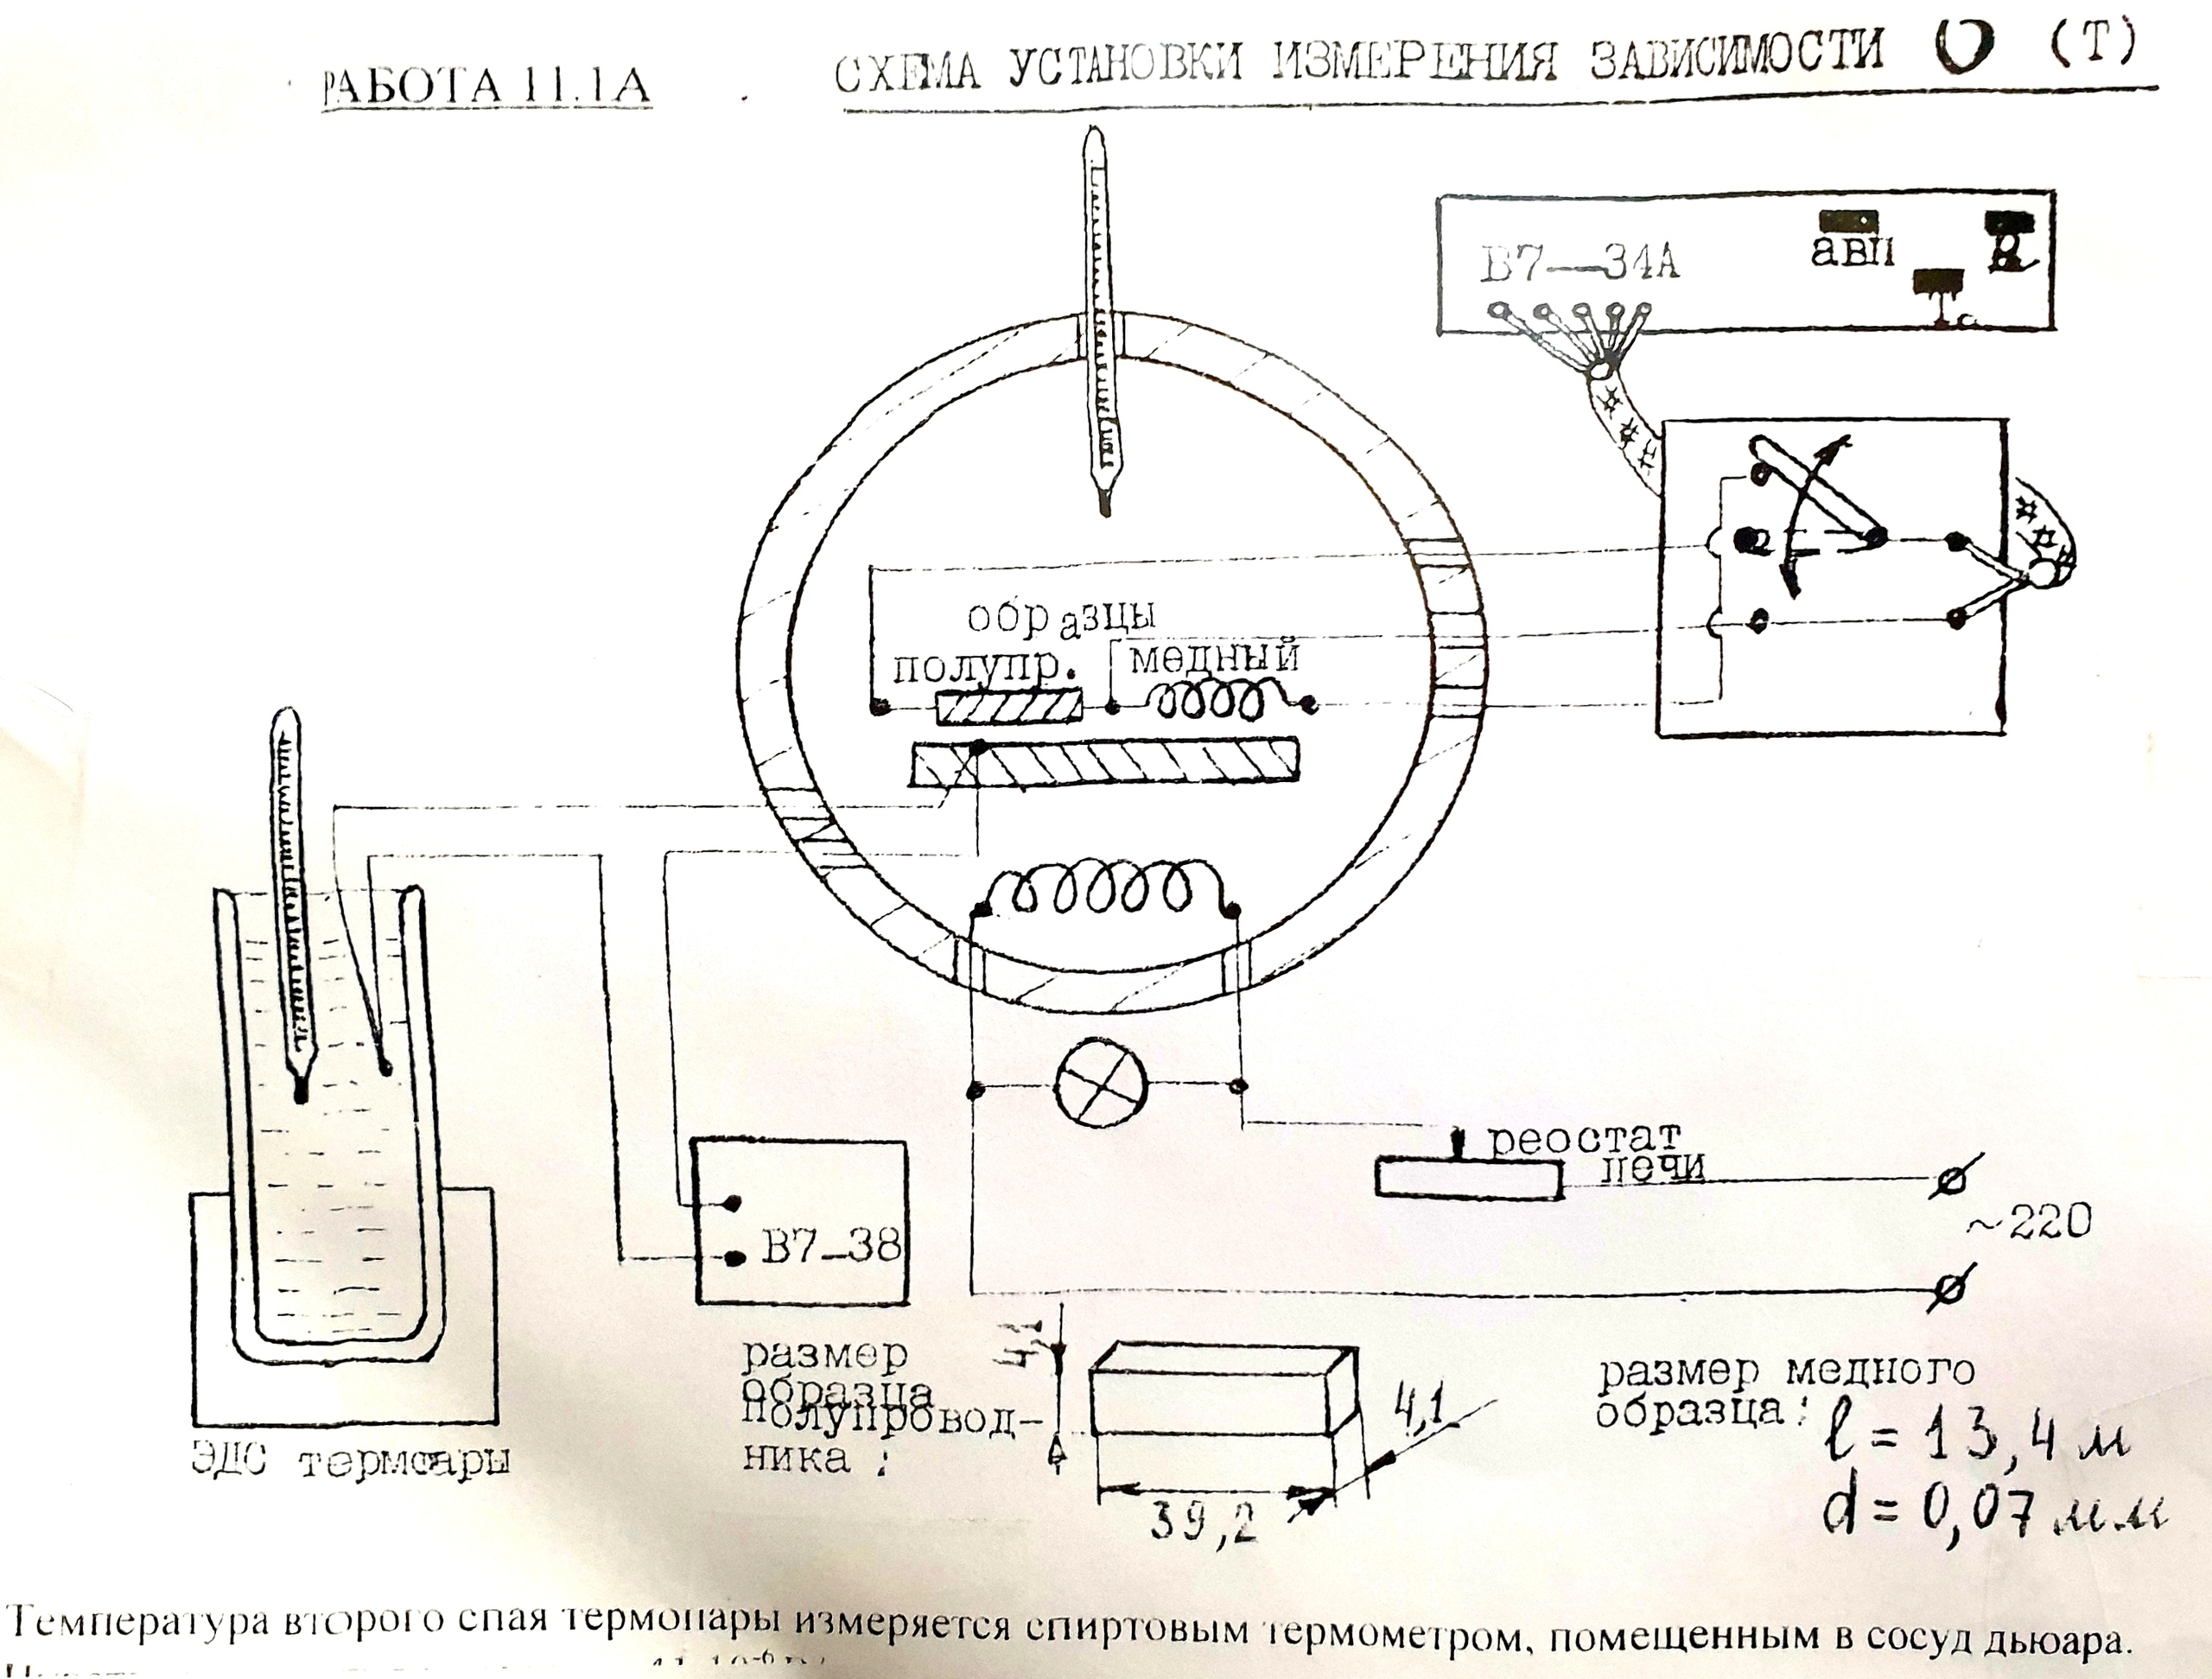
\includegraphics[width=0.8\textwidth]{UST}
\end{center}
\ECaption{Схема экспериментальной установки. Все необходимые параметры показаны на схеме.}
\end{figure}

Температура образцов определяется напряжением на термопаре, принимая во внимание комнатную температуру в 23$^{\circ}$С. Погрешность в определении температуры определяется приборной погрешностью вольтметра термопары -- 3 последних значащих цифры (0.03 мкВ). Аналогичная погрешность в измерении сопротивления образцов омметром (0.3 Ом).

Для цилиндрического образца проводимость определяется формулой:
\begin{equation}
\sigma = \dfrac{1}{\rho} = \frac{l}{RS}.
\end{equation}
\newpage
\section*{Выполнение эксперимента}

Экспериментальные данные представлены на таблице 1. Из нее можно понять, что с ростом температуры сопротивление образцов разных материалов меняется в противоположные стороны. Более наглядно эта зависимость изображена на графиках на рис.2.

\begin{table}[h]
\begin{center}
\begin{tabular}{|c|c|c|c|c|}
\hline
\rowcolor[HTML]{9698ED} 
$V_{\text{терм}}$, мкВ & $T$, $^{\circ}C$ & $\sigma_{T}$, м$^{\circ}C$ & $R_{\text{меди}}$, Ом & $R_{\text{пп}}$, Ом \\ \hline
440                    & 33               & 6.95             & 94.4                 & 448                 \\ \hline
\rowcolor[HTML]{9698ED} 
700                    & 41               & 4.49             & 96.5                 & 356.2               \\ \hline
1000                   & 48               & 3.21             & 98.7                 & 239.2               \\ \hline
\rowcolor[HTML]{9698ED} 
1200                   & 53               & 2.72             & 100.4                & 197.2               \\ \hline
1600                   & 63               & 2.10             & 103.6                & 137                 \\ \hline
\rowcolor[HTML]{9698ED} 
1900                   & 70               & 1.81             & 106                  & 105.5               \\ \hline
2200                   & 77               & 1.59             & 108.4                & 82.5                \\ \hline
\rowcolor[HTML]{9698ED} 
2600                   & 86               & 1.38             & 111.5                & 65                  \\ \hline
2900                   & 93               & 1.26             & 113.9                & 50                  \\ \hline
\rowcolor[HTML]{9698ED} 
3100                   & 97               & 1.19             & 115.3                & 43.5                \\ \hline
3400                   & 104              & 1.11             & 117.6                & 37.3                \\ \hline
\end{tabular}
\ECaption{Экспериментальные данные зависимости сопротивления образцов полупроводника и меди. Погрешность для температуры, связанная с методом определения температуры по напряжению на термопаре, представлена отдельным столбцом.}
\end{center}
\end{table}


\begin{figure}[h!]
\begin{minipage}[h]{0.53\linewidth}
\center{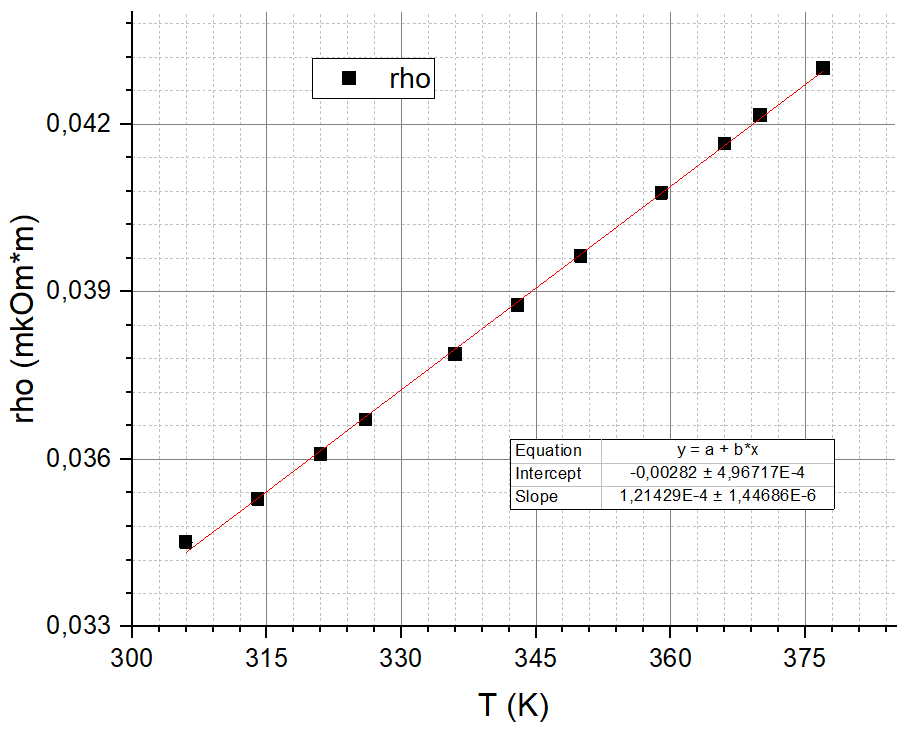
\includegraphics[width=1\linewidth]{gr1} \\ (a)}
\end{minipage}
\hfill
\begin{minipage}[h]{0.53\linewidth}
\center{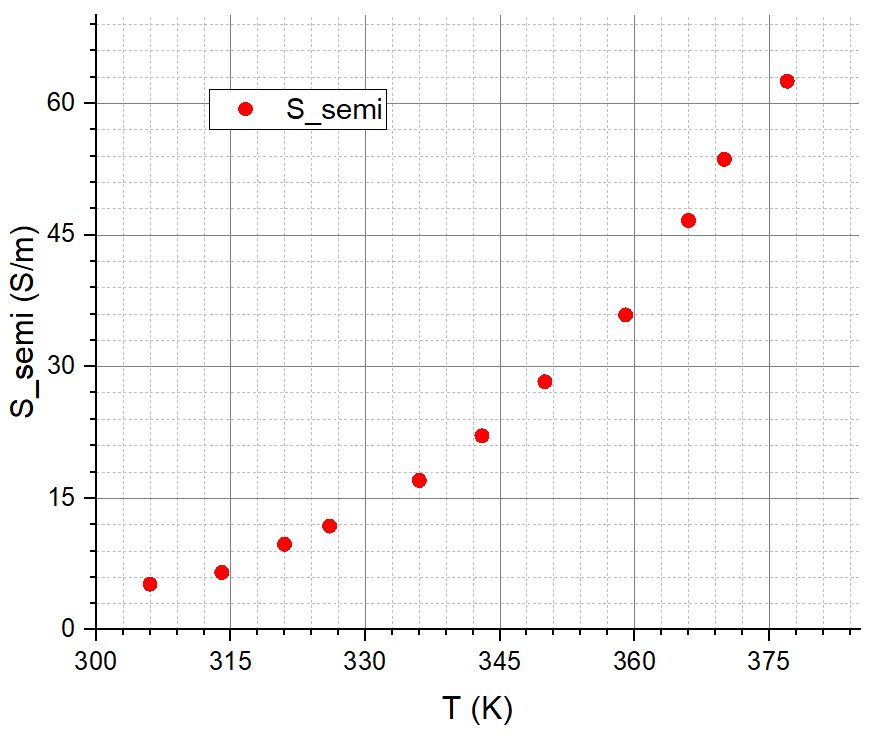
\includegraphics[width=1\linewidth]{gr2} \\ (б)}
\end{minipage}
\ECaption{a) График зависимости $\rho_{\text{м}}(T)$ -- удельного сопротивления меди от температуры (в мкОм$\cdot$м) б) График $\sigma_{\text{пп}}(T)$ -- полупроводника от температуры (в См/м)}
\end{figure}

Зависимости согласуются с теорией проводимости для своего материала. Проводимость меди уменьшается с ростом температуры (то есть удельное сопротивление растет), так как усиливаются тепловые колебания ионов решетки, а так же хаотическое движение самих электронов, что препятствует свободному движению зарядов. В полупроводниках же, наоборот, с увеличением температуры растет кол-во носителей заряда, из-за чего проводимость пп увеличивается.
\subsection*{Температурный коэффициент меди}

Из графика 2.а) можно получить уравнение аппроксимируещей прямой: $ \rho = I + S\cdot T  $. Тогда, если принять расчет для $\alpha$ из уравнения (7) для начальной температуры в 20$^{\circ}$C, то $\rho_0 = I+S\cdot 293$. Окончательно получаем:
\[\alpha = \dfrac{S}{I+293S} = 3.7 \pm 0.7 \text{ }\frac{\text{нОм}cdot\text{м}}{K},\]
где погрешность посчитана по следующей формуле:
\[\sigma_{\alpha} = \alpha*\sqrt{\left( \frac{\sigma_I}{I}\right)^2 + 2\left(\frac{\sigma_S}{S} \right)^2}. \]

Учитывая, что в большинстве источников, температурный коэффициент в диапазоне 0-100$^{\circ}$ равен 4 нОм*м/К, то с учетом погрешности и зависимости $\alpha$ от технологии изготовления меди, результаты можно считать достоверными.

\subsection*{Ширина запрещенной зоны полупроводника}

Линеаризовать график проводимости полупроводника от температуры можно в координатах Аррениуса (6). Полученный график изображен на рис.3.

\begin{figure}[h]
\begin{center}
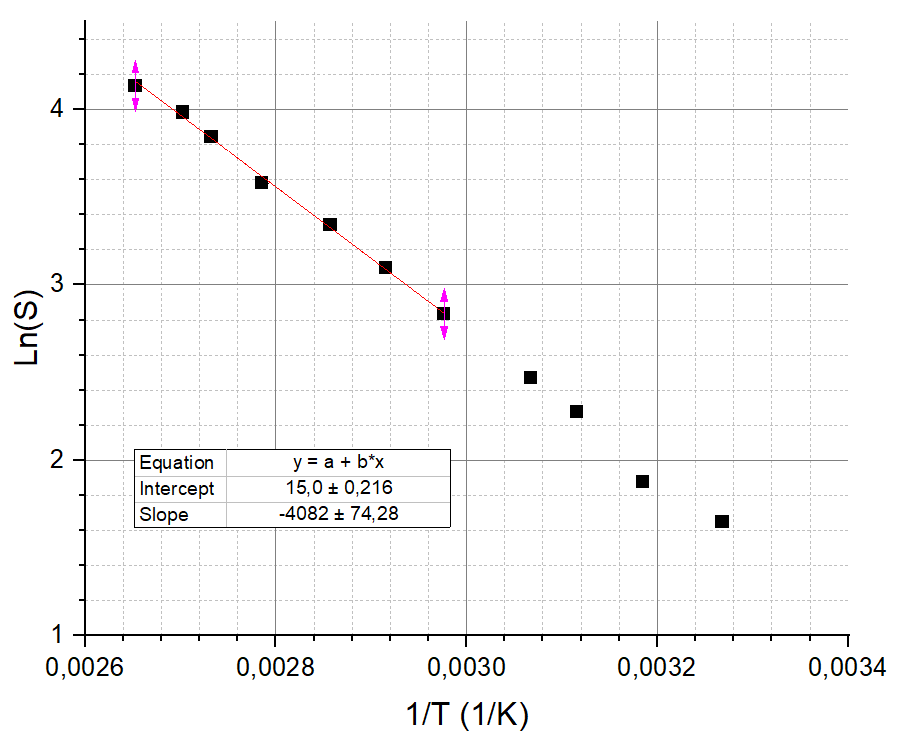
\includegraphics[width=0.9\textwidth]{gr3}
\end{center}
\ECaption{Линеаризованный график зависимости $ln(\sigma)\left( \frac{1}{T}\right)$. Аппрокисимрующая прямая построена по точкам из высокотемпературной области (первым 6). }
\end{figure}

Используя формулу (6) получаем, что ширина запрещенной зоны данного полупроводника при температурах, близких к комнатной, равна:
\[E_g = -2k\cdot S = 0.70 \pm 0.01 \text{ эВ}.\]

Известно, что при комнатной температуре ширина запрещенной зоны собственного полупроводника из германия (Ge) $E_{\text{Ge}}$ = 0.67 эВ. В работе исследовался собственный полупроводник, а т.к. найденная ширина находится в пределах 3 $\sigma$ от реального значения, то ислледуемый образец скорее всего состоит из германия. 
\newpage
\section*{Вывод}
Результаты можно считать достоверными, однако необходимо принять во внимания, что при данной методике измерения проводимость всегда будет немного занижена. Так как нагрев образца происходит непрерывно, то в момент измерения он еще не достигнет термодинамического равновесия с термопарой на всем своем объеме. Благодаря его малым размерам он нагревается достаточно быстро, однако для более точных измерений необходимо перед снятием данных ждать хотя бы пару минут на одной и той же температуре.








\end{document}